\documentclass[10pt,a4paper]{article}
\usepackage[utf8]{inputenc}
\usepackage[T1]{fontenc}
\usepackage{amsmath}
\usepackage{amsfonts}
\usepackage{amssymb}
\usepackage{natbib}
\usepackage{graphicx}

\title{Artificial Neural Networks (ANNs) Basic Theory}
\author{Max Cotton}
\date{}

\begin{document}

\maketitle

\section{Structure of an ANN:}

\begin{itemize}
    \item Input layer of multiple inputs/neurons (in an array)
    \item Hidden layers of calculations (the more layers, the more accurate the prediction), consisting of the following:
    \begin{itemize}
        \item An Activation function:
        \begin{itemize}
            \item Calculate the dot product of the input array with a hidden weight array, then sum the result with a bias
        \end{itemize}
        \item A Transfer function to get an output, Eg: Sigmoid function to transform the result of the Activation function to a number between 0 and 1, then the result can be classified as closer to 0 or 1 (known as logistic regression), with 0 being one state and 1 being another
    \end{itemize}
    \item Output layer to output the final result of the calculations from the hidden layers, consisting of the following:
    \begin{itemize}
        \item An Activation function:
        \begin{itemize}
            \item Caclulate the dot product of the hidden layer output with an output weight array, then sum the result with a bias
        \end{itemize}
        \item A Transfer function to get an output (round output to one end of range with a meaning)
    \end{itemize}
    \item Afterwards, the weights and the bias are all initialised to zero/s
\end{itemize}

\section{How ANNs are trained:}

\begin{itemize}
    \item Forward Propagation, the process of feeding inputs into the neural network and getting a result/prediction
    \item Back Propagation, the process of calculating the error in the prediction then adjusting the weights and biases accordingly, consisting of the following:
    \begin {itemize}
        \item A Cost/Loss function (used for graphs and deriving formula for gradient descent):
        \begin{itemize}
            \item Finds the average of the difference between the actual and the predicted value for each input
        \end{itemize}
        \item Gradient descent:
        \begin{itemize}
            \item Update the hidden/output weight arrays and bias, by subtracting the rate of change of Loss with respect to Weight, multiplied with a learning rate
            \item This repetitive process will continue to reduce the loss to a minimum, if the learning rate is set to an appropriate value
                \begin{figure}[h!]
                \centering
                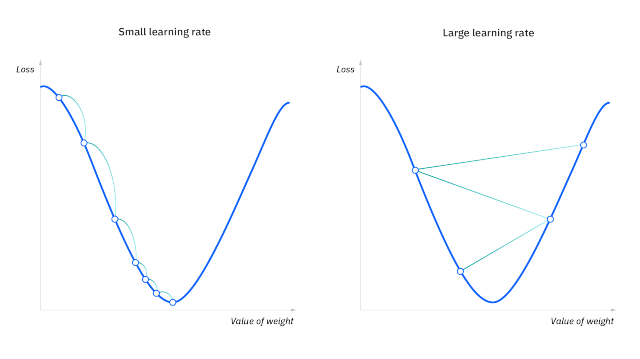
\includegraphics[width=1\textwidth]{./docs/models/src/images/gradient-descent.png}
                \caption{Gradient Descent\\
                         sourced from https://www.ibm.com/topics/gradient-descent}
                \end{figure}
        \end{itemize}
    \end{itemize}
\end{itemize}

\end{document}